\documentclass[accentcolor=tud9b, colorbacktitle, inverttitle]{tudbeamer}

\usepackage[utf8]{inputenc}
\usepackage[T1]{fontenc}
\usepackage[ngerman]{babel}
\usepackage{epstopdf}
\usepackage{graphicx}
\usepackage{xcolor}
\usepackage{tikz}
\usepackage{lipsum,multicol}
% \usepackage[backend=biber]{biblatex}
% \addbibresource{References_PSBeschl_2018.bib}

% style=alphabetic, 
\usepackage{tikz}						% graphics creation environment frontend
\usepackage{tikz-cd}
\usepackage{import}
\usepackage{multicol}
\usepackage{subfig}
% 
\usepackage{pgfplots}					% graph plotting for pgf/tikz
\pgfplotsset{compat=1.12, grid style={gray,dotted}}

% \usetikzlibrary{external} %% comment out to stop externalization of tikz pictures
% \tikzexternalize[optimize=false, prefix=tikz-external/] % path to store the externalized stuff in
% \tikzset{external/system call={lualatex \tikzexternalcheckshellescape -halt-on-error-interaction=batchmode -jobname "\image" "\texsource"}, force remake = false}
% % \tikzset{external/force remake = false}
% \tikzexternalize

\graphicspath{{graph/}}

\author{Julian Buschbaum, Benjamin Northe, Rainer Stellnberger}
\institute{Institut TEMF~\textbar~Fachgebiet Beschleunigertechnik}
\logo[1.5]{\includegraphics{temf}}
\date{28. September 2018}
\title{Untersuchungen zur Impedanzreduktion an MA-Kavitäten durch Kurzschließen von Ringkernen \vspace{0.2em}}
\subtitle{Betreuer: Jens Schweickhardt, M.Sc.\\ Fachgebietsleiter: Prof. Dr.-Ing. Harald Klingbeil}

\begin{document}

\begin{titleframe}
\vspace{-1em}
	\begin{figure}[h]
		\centering
		\includegraphics[width=0.625\textwidth]{Kavitaet}
	\end{figure}
\end{titleframe}





\begin{frame}\frametitle{Inhalt}
	\begin{itemize}
		\item Aufgabenstellung
		\item Der Messaufbau
		\item Simulation
		\item Gegen\"uberstellung der Messung und Simulation
		\item Auswertung der Kurzschlussanordnungen
		\item Fazit und Ausblick
	\end{itemize}
\end{frame}


\begin{frame}\frametitle{Aufgabenstellung}
\begin{multicols}{2}
\vspace{-2em}
	\begin{figure}[h]
		\centering
		\includegraphics[width=0.5\textwidth]{Kavitaet}
	\end{figure}
	\vfill\null
	\columnbreak
	\begin{itemize}
		\item MA(Magnetic Alloy)-Ringkerne zur Stimmung der Kavit\"at
		\item Im passiven Betrieb der Kavit\"at m\"oglichst wenig Einfluss auf den Strahl gewünscht (Impendanz)
		\item Theorie: Kurzschlussschaltung um die Ringkerne soll deren Einfluss auf die Impedanz reduzieren
	\end{itemize}
\end{multicols}
\end{frame}


\begin{frame}\frametitle{Die Testbox}
% \vspace{-2em}
% 	\begin{figure}[h]
% 		\centering
% 		\includegraphics[width=0.72\textwidth]{opentest}
% 	\end{figure}
\end{frame}


\begin{frame}\frametitle{Konstruktion der Ringkernhalterung}
 
\end{frame}


\begin{frame}\frametitle{Entwurf der Kurzschlussschienen}
 
\end{frame}




\begin{frame}\frametitle{Messdurchf\"uhrung}
% \begin{multicols}{2}
% 	\vspace{-2em}
% 	\begin{figure}[h]
% 		\centering
% 		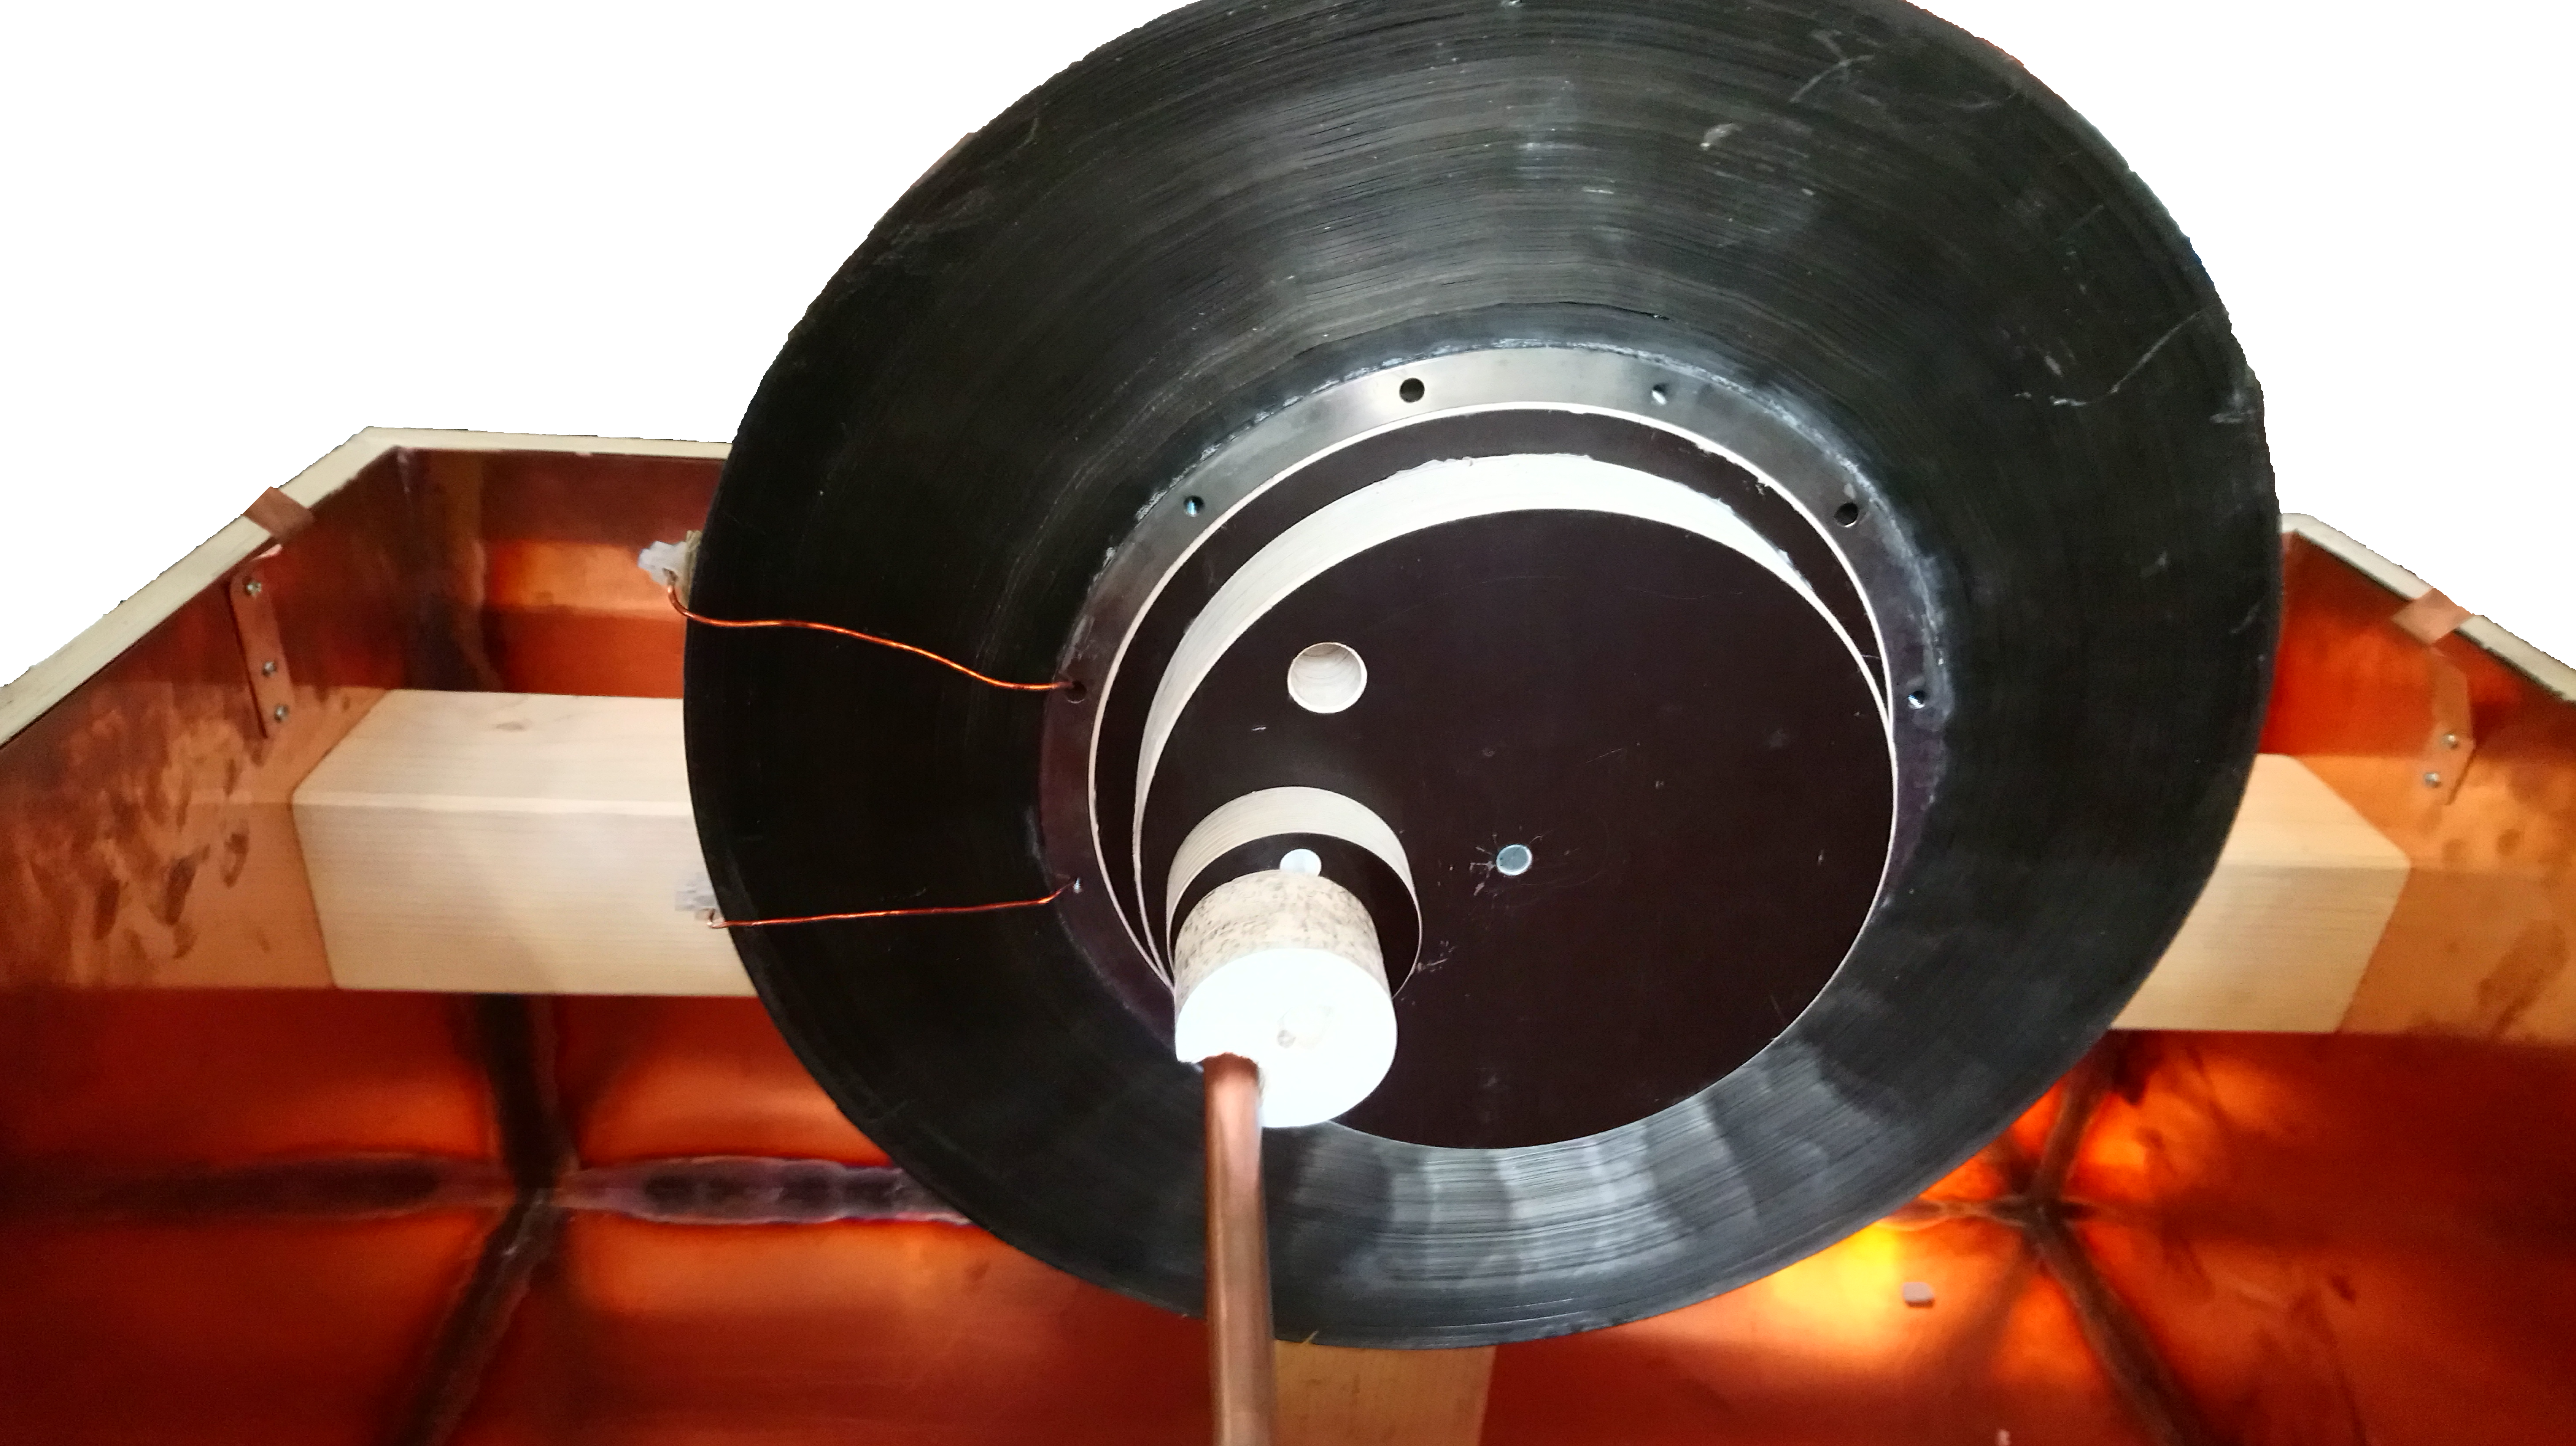
\includegraphics[width=0.5\textwidth]{test_ks_adapted_v2}
% 	\end{figure}
% 	\vfill\null
% 	\columnbreak
% 	\begin{itemize}
% 		\item Fixierung der Kurzschl\"usse schwierig
% 		\item Messung dadurch nur bedingt reproduzierbar
% 	\end{itemize}
% \end{multicols}
\end{frame}






\begin{frame}\frametitle{Simulation}
% Mithilfe von CST wurden mehrere Faktoren f\"ur die Kurzschl\"usse durchsimuliert:
% \begin{itemize}
% 	\item Anzahl der Kurzschl\"usse
% 	\item Positionen der Kurzschl\"usse
% 	\item Formen der Kurzschl\"usse
% 	\item Verschiedene Abst\"ande der Kurzschlusswicklung zum Ringkern
% 	\item Feldimpedanz mit einer unterbrochenen Schiene (wenn sich diese im Leerlauf befindet)
% \end{itemize}
\end{frame}


\begin{frame}\frametitle{Realit\"atsgetreue Anpassungen der Simulation}

\end{frame}



\begin{frame}\frametitle{Ringkernmodellierung}

\end{frame}



\begin{frame}\frametitle{Simualtionsdurchf\"uhrung}

\end{frame}



\begin{frame}\frametitle{Gegen\"uberstellung der Simulations- und Messergebnisse}

\end{frame}



\begin{frame}\frametitle{Auswertung der Kurzschlussanordnungen}

\end{frame}



\begin{frame}\frametitle{Simualtionsdurchf\"uhrung}

\end{frame}





\begin{frame}\frametitle{Anzahl der Kurzschl\"usse}
% \vspace{-2em}
% \begin{figure}[h]
% 	\subfloat[]{\includegraphics[height = 0.3\textwidth]{1ksTorus}} \hspace{1em}
% 	\subfloat[]{\includegraphics[height = 0.3\textwidth]{4ksTorus}}\hspace{1em}
% 	\subfloat[]{\includegraphics[height = 0.3\textwidth]{24ksTorus}}
% \end{figure}
\end{frame}



\begin{frame}\frametitle{Breite der Kurzschlüsse}
% \vspace{-2em}
% \begin{figure}[h]
% 	\subfloat[]{\includegraphics[height = 0.4\textwidth]{4ksTorus}} \hspace{1em}
% 	\subfloat[]{\includegraphics[height = 0.4\textwidth]{4ksTorus30Grad}}
% \end{figure}
\end{frame}


\begin{frame}\frametitle{Länge der Kurzschlüsse}
% \vspace{-2em}
% \begin{figure}[h]
% 	\subfloat[]{\includegraphics[height = 0.3\textwidth]{1ksTorus}} \hspace{1em}
% 	\subfloat[]{\includegraphics[height = 0.3\textwidth]{1ksSchiene}}\hspace{1em}
% 	\subfloat[]{\includegraphics[height = 0.3\textwidth]{1ksSchieneSchmal}}
% \end{figure}
\end{frame}


\begin{frame}\frametitle{Dicke der Kurzschlüsse}
% \vspace{-2em}
% \begin{figure}[h]
% 	\centering
% 	\includegraphics[width=0.45\textwidth]{1ksSchieneWeit}
% \end{figure}
\end{frame}




\begin{frame}\frametitle{Einfluss im Leerlauf befindlicher Schienen auf die Ringkernimpedanz}
% \vspace{-2em}
% \begin{figure}[h]
% 	\centering
% 	\includegraphics[width=0.35\textwidth]{1ksSchieneOffen}
% \end{figure}
\end{frame}



\begin{frame}\frametitle{Fazit und Ausblick}
% Was steht jetzt noch an:
%         \begin{itemize}
%             \item Montage der neuen Halterung
%             \item Messung der simulierten Kurzschlussanordnungen
%             \item Vergleich von Simulation und Messung
%             \item Bewertung der Einflussfaktoren
%             \item Ausarbeiten einer favorisierten Umsetzung der Kurzschlussanordnung
%             \item Übertragen der Teststandmessung auf die Breitbandkavität
%             
%         \end{itemize}

\end{frame}

% \begin{frame}\frametitle{Quellen}
% % 	\bibliographystyle{plain}
% 	\bibliography{References_PSBeschl_2018.bib} 
% \end{frame}



\end{document}
